% Provenance (never printed): see sources/outline_sources.md (Year 1: the carbonate factory;
% reefs and platforms; pelagic oozes and the carbonate compensation depth; siliceous oozes;
% evaporite sequences). Exercise and problem values in the Book 3 scratch calculator
% calc/ch22.py; figure data from figdata/bachelor-1/evaporation.py and ccd_flank.py.
% Calcite, aragonite and dolomite are ch. 7's; the depth--age law ch. 13's; salinity Book 1's
% (g8); limestone Book 1's (g6, prose); the carbonate system and alkalinity the chemistry and
% biology books' (recalled, never defined). The subsidence of volcanic islands under reefs is
% the Year 2 volume's (oceanic islands); diagenesis (dolomitisation, chert, gypsum to
% anhydrite) is ch. 23's; upwelling ch. 29's.
\chapter{Les sédiments carbonatés, siliceux et évaporitiques}\label{ch:b1:chemical-biogenic-sediments}

Les falaises de craie blanche qui se font face de part et d'autre du bras de mer
étroit entre l'Angleterre et la France ressemblent à la plus ordinaire des
roches. Au microscope électronique, elles se révèlent faites d'innombrables
minuscules plaques de calcite, lâchées par des algues unicellulaires qui
flottaient dans la mer qui couvrait la région. Un \omterm{def:b1:chemical-biogenic-sediments:reef}{récif} vu d'un bateau raconte
la même histoire à l'autre bout de l'échelle~: un calcaire en train de se faire,
bâti par des coraux et des algues qui prennent à l'eau le calcium et le
carbonate pour en faire de la pierre. Tous les sédiments ne sont pas apportés~;
beaucoup se fabriquent là où ils reposent, par des êtres vivants ou par l'eau
elle-même quand elle s'évapore. Ce chapitre suit les trois grandes familles de
ces sédiments --- carbonates, \omterm{def:b1:chemical-biogenic-sediments:ooze}{vases siliceuses} et \omterm{def:b1:chemical-biogenic-sediments:evaporite}{évaporites} --- depuis la
chimie de la mer qui les nourrit jusqu'aux roches qu'ils laissent.

\begin{recall}
Le calcaire est une roche sédimentaire faite de calcite, souvent issue de
coquilles, et il fait effervescence dans un acide dilué (livre~1, année~6). La
calcite et l'aragonite sont les deux \omterm{def:b1:rock-forming-minerals:polymorph}{polymorphes} de \ce{CaCO3}, de masses
volumiques \qty{2.71}{g.cm^{-3}} et \qty{2.93}{g.cm^{-3}}, et la dolomite
\ce{CaMg(CO3)2}, de masse volumique \qty{2.84}{g.cm^{-3}}, est le carbonate de
calcium et de magnésium (\cref{ch:b1:rock-forming-minerals}). La salinité de
l'eau de mer est la masse de sel dissous dans un kilogramme de cette eau
(livre~1, année~8). Dans l'eau, le dioxyde de carbone, l'ion hydrogénocarbonate
et l'ion carbonate sont liés par des équilibres acide--base, et l'alcalinité
mesure les bases capables de capter des ions hydrogène (les livres de chimie)~;
le système des carbonates de l'océan prend part au cycle du carbone (les livres
de biologie). Le fond marin s'approfondit avec l'âge selon $d = d_r + C\sqrt t$
(\cref{thm:b1:rifts-ridges-margins:depth-age}).
\end{recall}
% ledger: webmineral:polymorphs, hom:calcite, webmineral:others

\section{L'usine à carbonates}\label{sec:b1:chemical-biogenic-sediments:factory}

L'eau de mer contient du calcium et du carbone inorganique dissous, surtout sous forme
d'hydrogénocarbonate. Le carbonate de calcium se forme à partir d'eux par les réactions
\[
\ce{Ca^2+ + 2 HCO3- -> CaCO3 + CO2 + H2O}, \qquad
\ce{Ca^2+ + CO3^2- -> CaCO3},
\]
la première libérant une molécule de dioxyde de carbone pour chaque unité de carbonate
déposée. L'eau chaude de surface des tropiques est sursaturée en carbonate de
calcium, mais celui-ci précipite rarement de lui-même~: presque tout est fabriqué
par des êtres vivants, qui dépensent l'énergie nécessaire pour bâtir leurs
coquilles et leurs squelettes et qui commandent le \omterm{def:b1:rock-forming-minerals:mineral}{minéral} qu'ils emploient. Les
coraux et les algues vertes bâtissent de l'aragonite~; les algues rouges et de
nombreux foraminifères bâtissent de la calcite, en partie riche en magnésium~;
les mollusques utilisent l'une, l'autre ou les deux.

\begin{definition}[Usine à carbonates]\label{def:b1:chemical-biogenic-sediments:factory}
L'\emph{usine à carbonates}\index{usine a carbonates@usine à carbonates} d'une mer est l'ensemble des
organismes et des processus qui produisent du sédiment de carbonate de calcium là où on le
trouve, plutôt que de l'apporter d'ailleurs. Ses produits sont des grains squelettiques
(coquilles et squelettes entiers ou brisés), de la boue carbonatée, des grains enrobés et les
charpentes rigides des \omterm{def:b1:chemical-biogenic-sediments:reef}{récifs}.
\end{definition}

L'usine la plus riche travaille dans une eau chaude, claire, peu profonde et ensoleillée, loin
de la boue des rivières, qui enterrerait les producteurs et troublerait la lumière dont les
algues ont besoin. Son sédiment est fabriqué par le fond marin lui-même~: débris de coraux
et d'algues, coquilles de mollusques et de foraminifères unicellulaires qui vivent
sur le fond, et aiguilles d'aragonite lâchées par les algues vertes, qui se déposent en une
boue carbonatée. Là où l'eau est agitée et sursaturée, des grains roulés par
les vagues et les marées se couvrent d'enveloppes de carbonate, couche après couche, autour d'un noyau,
un grain de sable ou un fragment de coquille, et deviennent de ronds \omterm{def:b1:chemical-biogenic-sediments:reef}{ooïdes}
(\cref{def:b1:chemical-biogenic-sediments:reef}). Une seconde usine travaille en
plein océan, loin de tout rivage~: le plancton de la couche de surface ensoleillée
bâtit de minuscules coquilles et plaques de calcite qui pleuvent jusqu'au fond de la mer profonde
(\cref{sec:b1:chemical-biogenic-sediments:oozes}).
% ledger: og:carbonates

La vitesse à laquelle une usine bâtit se mesure par son bilan de carbonate, la masse de
carbonate produite et conservée sur place chaque année sur un mètre carré, après
les pertes dues aux organismes perforants, aux brouteurs et aux vagues. Il se traduit en une
vitesse verticale de croissance par un bilan de masse.

\begin{proposition}[Accrétion à partir d'un bilan de carbonate]\label{prop:b1:chemical-biogenic-sediments:accretion}
Soit un fond marin qui conserve sur place la masse nette $G$ de carbonate de calcium par unité d'aire
et de temps, sous forme d'un dépôt dont les grains solides ont la masse volumique $\rho_s$
et dont la porosité, la fraction de son volume occupée par les pores, vaut $\phi$. Alors
le fond s'élève à la vitesse
\[
a = \frac{G}{\rho_s\,(1-\phi)}.
\]
\end{proposition}

\begin{proof}
Pendant le temps $\mathrm dt$, une unité d'aire reçoit la masse $G\,\mathrm dt$ de
carbonate solide, qui remplit le volume $G\,\mathrm dt/\rho_s$ de grains. Ces
grains forment la fraction $1-\phi$ de la nouvelle couche, dont l'épaisseur est
donc $G\,\mathrm dt/(\rho_s(1-\phi))$. En divisant par $\mathrm dt$, on obtient $a$.
\end{proof}

Le produit $\rho_s(1-\phi)$ est la masse volumique sèche apparente du dépôt. Sur
les \omterm{def:b1:chemical-biogenic-sediments:reef}{récifs} de l'archipel des Chagos, dans l'océan Indien, 28 \omterm{def:b1:chemical-biogenic-sediments:reef}{récifs} mesurés en 2015
avaient un bilan moyen de \qty{3.7}{kg} de \ce{CaCO3} par mètre carré et par
an, et ceux que dominent les coraux ramifiés \emph{Acropora} \qty{8.4}{kg},
pour une croissance d'environ \qty{4.2}{mm} par an~; avec la proposition, ces deux nombres
indiquent ensemble une masse volumique sèche apparente de \qty{2000}{kg.m^{-3}}, c'est-à-dire une
charpente de \omterm{def:b1:chemical-biogenic-sediments:reef}{récif} faite pour un tiers environ d'espace poreux (\cref{exo:b1:chemical-biogenic-sediments:3}).
Ces mêmes \omterm{def:b1:chemical-biogenic-sediments:reef}{récifs} avaient perdu plus de neuf dixièmes de leurs coraux lors de l'épisode de
réchauffement de 1998, et leurs bilans montrent la vitesse à laquelle un \omterm{def:b1:chemical-biogenic-sediments:reef}{récif} peut se reconstruire.
% ledger: perry:chagos

\section{Récifs et plates-formes}\label{sec:b1:chemical-biogenic-sediments:reefs}

Là où l'usine bâtit une charpente rigide, celle-ci peut se dresser sur le fond marin
face aux vagues.

\begin{definition}[Récif, plate-forme carbonatée, ooïde]\label{def:b1:chemical-biogenic-sediments:reef}
Un \emph{récif}\index{recif@récif} est un édifice carbonaté dont la charpente d'organismes,
coraux, algues ou autres, qui ont crû sur place et se sont liés et cimentés, se dresse
au-dessus du fond marin environnant et résiste aux vagues. Une \emph{plate-forme
carbonatée}\index{plate-forme carbonatee@plate-forme carbonatée} est un épais corps de carbonate
de faible profondeur dont le sommet plat se trouve près du niveau de la mer et qui est limité par une pente vers
des eaux plus profondes. Un \emph{ooïde}\index{ooide@ooïde} est un grain rond de la taille d'un sable, fait de
couches concentriques de carbonate de calcium développées autour d'un noyau qui roulait dans
une eau agitée~; une roche faite d'ooïdes est une oolithe.
\end{definition}
% ledger: og:carbonates

Les \omterm{def:b1:chemical-biogenic-sediments:reef}{récifs} coralliens actuels sont de trois sortes, nommées par les voyageurs qui les ont cartographiés
bien avant que personne en ait traversé un par forage. Un \omterm{def:b1:chemical-biogenic-sediments:reef}{récif} \emph{frangeant} est attaché à
la côte d'une île ou d'un continent. Un \omterm{def:b1:chemical-biogenic-sediments:reef}{récif} \emph{barrière} est séparé de
la terre par un lagon, qui peut être large et profond de plusieurs dizaines de mètres~: la barrière
au large du nord-est de l'Australie court, avec des interruptions, sur près de mille milles,
et enferme une mer profonde de 10 à 25 brasses, soit environ 18 à \qty{46}{m}. Un
\emph{atoll} est un anneau de \omterm{def:b1:chemical-biogenic-sediments:reef}{récif}, portant de basses îles de sable corallien, autour d'un
lagon qui ne contient aucune terre.

\begin{omfigure}
\begin{tikzpicture}[font=\footnotesize, scale=0.72]
% three reef types in cross-section (schematic): a volcanic cone y = 2 - s - 0.75|x - 4|
% subsided by s (0, 0.8, 1.6), sea level at y = 1; the reef grows up from its first
% position, the foot of the fringing reef at (2, 0.5) moving down with the cone
\foreach \s/\yo/\lab/\name in {0/0/a/récif frangeant, 0.8/-3.8/b/récif barrière, 1.6/-7.6/c/atoll} {
  \begin{scope}[yshift=\yo cm]
    \begin{scope}
      \clip (0,-1.3) rectangle (8,2.3);
      \fill[omSea] (0,-1.3) rectangle (8,1.0);
      \draw[lith basalt] (-1,2-\s-3.75) -- (4,2-\s) -- (9,2-\s-3.75) -- cycle;
    \end{scope}
    \draw[omSea!60!black] (0,1.0) -- (8,1.0);
    \node[anchor=west, font=\scriptsize, align=left] at (8.05,1.0) {niveau\\ de la mer};
    \node[anchor=west] at (0,2.05) {(\lab) \name};
    \draw[black!70] (1.05,1.55) node[anchor=east, font=\scriptsize] {récif} -- (2.2,1.02);
  \end{scope}
}
% (a) fringing reef: wedges against the shore
\fill[lith reef limestone, draw=black!70] (2.0,0.5) -- (2.15,1.0) -- (2.667,1.0) -- cycle;
\fill[lith reef limestone, draw=black!70] (6.0,0.5) -- (5.85,1.0) -- (5.333,1.0) -- cycle;
\node[anchor=west, font=\scriptsize] at (4.9,1.75) {île volcanique};
% (b) barrier reef: the cone has sunk by 0.8, the reef has grown up, a lagoon opens
\begin{scope}[yshift=-3.8cm]
  \fill[lith reef limestone, draw=black!70] (2.0,-0.3) -- (2.15,1.0) -- (2.6,1.0) -- (2.55,0.1125) -- cycle;
  \fill[lith reef limestone, draw=black!70] (6.0,-0.3) -- (5.85,1.0) -- (5.4,1.0) -- (5.45,0.1125) -- cycle;
  \draw[black!70] (3.2,0.85) -- (3.7,1.45) node[anchor=west, font=\scriptsize, inner sep=1pt] {lagon};
\end{scope}
% (c) atoll: the cone has sunk by 1.6 and is drowned; the reef ring encloses a lagoon
\begin{scope}[yshift=-7.6cm]
  \fill[lith limestone, draw=black!50] (2.55,-0.6875) -- (2.55,0.55) -- (5.45,0.55) -- (5.45,-0.6875) -- (4,0.4) -- cycle;
  \fill[lith reef limestone, draw=black!70] (2.0,-1.1) -- (2.15,1.0) -- (2.6,1.0) -- (2.55,-0.6875) -- cycle;
  \fill[lith reef limestone, draw=black!70] (6.0,-1.1) -- (5.85,1.0) -- (5.4,1.0) -- (5.45,-0.6875) -- cycle;
  \node[font=\scriptsize] at (4,0.78) {lagon};
  \node[font=\scriptsize, fill=omLithLime, inner sep=1pt] at (4,0.05) {sédiment de lagon};
\end{scope}
% photograph
\node[anchor=north west, inner sep=0] at (10.75,2.3) {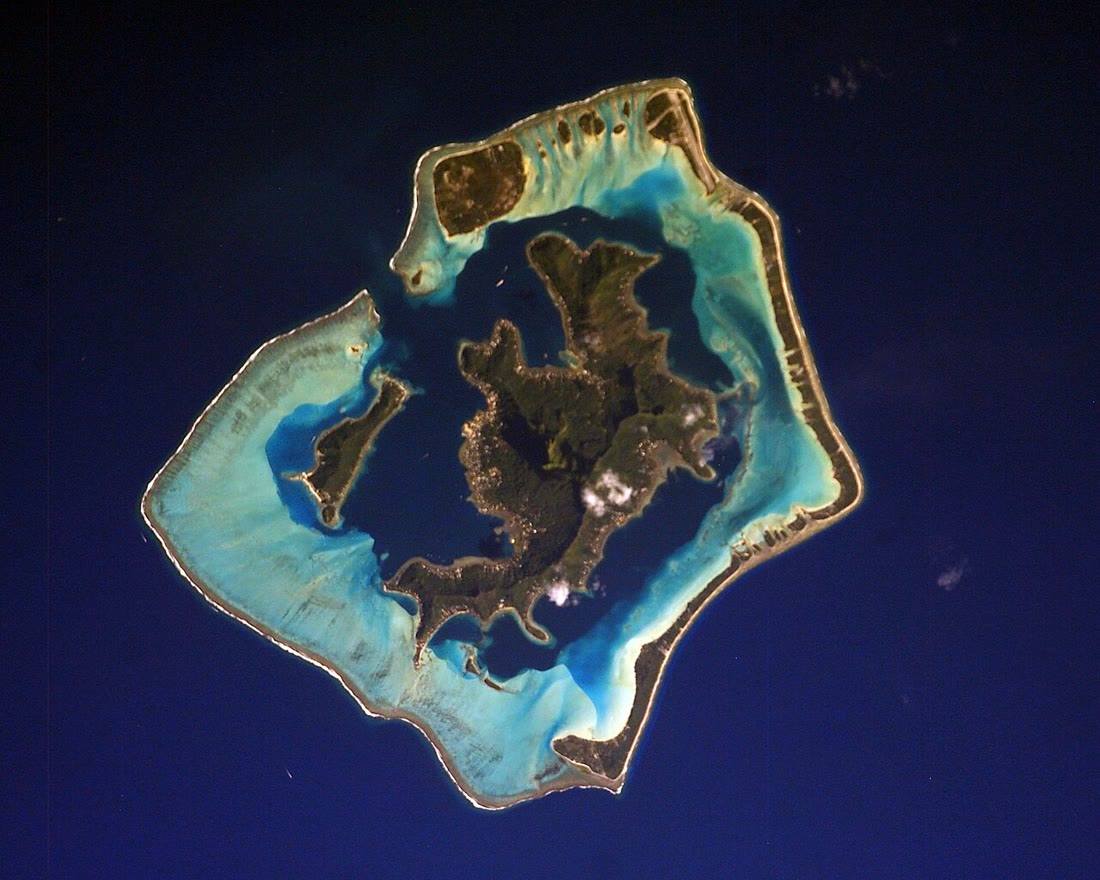
\includegraphics[height=6.9cm]{images/book3/b1-bora-bora.jpg}};
\end{tikzpicture}

{\small À gauche~: les trois sortes de \omterm{def:b1:chemical-biogenic-sediments:reef}{récif} corallien en coupe (schématique,
échelle verticale très exagérée), dessinées comme Darwin les a expliquées~: (a)~un \omterm{def:b1:chemical-biogenic-sediments:reef}{récif}
frangeant une île volcanique~; (b)~l'île s'est enfoncée et le \omterm{def:b1:chemical-biogenic-sediments:reef}{récif}, croissant
vers le haut, est devenu une barrière séparée de la côte par un lagon~; (c)~
l'île a disparu sous les eaux et le \omterm{def:b1:chemical-biogenic-sediments:reef}{récif} est un atoll autour d'un lagon au fond tapissé
de sédiment carbonaté. À droite~: Bora Bora, île volcanique dans un lagon
enclos par un \omterm{def:b1:chemical-biogenic-sediments:reef}{récif} barrière portant de basses îles, photographiée par un astronaute
depuis la Station spatiale internationale le 19~mars 2003 (NASA, domaine public,
via Wikimedia Commons).}
\label{fig:b1:chemical-biogenic-sediments:reefs}
\end{omfigure}
% ledger: darwin:reefs, commons:bora-bora

\begin{history}[Les récifs sur des fondations qui s'enfoncent, 1837--1842]
Au cours du voyage du \emph{Beagle}, Charles Darwin navigua parmi
les \omterm{def:b1:chemical-biogenic-sediments:reef}{récifs} des océans Pacifique et Indien. Il partit d'un seul fait~: les coraux bâtisseurs de \omterm{def:b1:chemical-biogenic-sediments:reef}{récifs}, conclut-il, ne
prospèrent pas en général plus profond qu'entre 20 et 30 brasses, soit environ 37 à \qty{55}{m}.
Pourtant les \omterm{def:b1:chemical-biogenic-sediments:reef}{récifs} barrières et les atolls s'élèvent depuis des eaux profondes, bien en dessous de cette limite. Leurs
fondations, soutint-il, devaient s'être enfoncées, assez lentement pour que les coraux gardent
leur sommet à la surface en croissant vers le haut~: un \omterm{def:b1:chemical-biogenic-sediments:reef}{récif} qui frange une île
volcanique devient une barrière quand l'île s'enfonce derrière lui, et un atoll quand
l'île a disparu. Il lut sa théorie devant la Société géologique de
Londres le 31 mai 1837 et la publia en 1842 dans \emph{The Structure and
Distribution of Coral Reefs}, avec une carte de tous les \omterm{def:b1:chemical-biogenic-sediments:reef}{récifs} du monde classés
en trois sortes. Pourquoi les îles océaniques s'enfoncent, et de combien, tient au
refroidissement de la plaque qui les porte, traité dans le volume de deuxième année.
\end{history}
% ledger: darwin:reefs

Un \omterm{def:b1:chemical-biogenic-sediments:reef}{récif} ne survit que si son sommet reste dans l'eau peu profonde où vivent ses
bâtisseurs. Le niveau de la mer change, et la fondation peut s'enfoncer~; ce qui compte est la
somme des deux, la montée relative du niveau de la mer.

\begin{proposition}[Suivre ou se noyer]\label{prop:b1:chemical-biogenic-sediments:keep-up}
Soit le sommet d'un \omterm{def:b1:chemical-biogenic-sediments:reef}{récif} à la profondeur $D_0$ sous le niveau de la mer, croissant vers le haut à
la vitesse $a$, tandis que le niveau relatif de la mer monte à la vitesse $r$, toutes deux
constantes. Alors la hauteur d'eau au-dessus du \omterm{def:b1:chemical-biogenic-sediments:reef}{récif} après le temps $t$ est
\[
D(t) = D_0 + (r - a)\,t .
\]
Si $a \ge r$, le \omterm{def:b1:chemical-biogenic-sediments:reef}{récif} suit la mer (quand $a > r$ son sommet atteint la
surface, et il ne peut plus ensuite croître que latéralement)~; si $a < r$ il prend
du retard, et si ses bâtisseurs ne peuvent vivre plus profond que $D_{\max}$, il se noie après
le temps $(D_{\max} - D_0)/(r - a)$.
\end{proposition}

\begin{proof}
Mesurons les hauteurs vers le haut à partir d'un repère fixe de la fondation. Le sommet du \omterm{def:b1:chemical-biogenic-sediments:reef}{récif}
est à $h_0 + a t$ et la surface de la mer à $s_0 + r t$, donc la hauteur d'eau au-dessus
du sommet est $D = (s_0 - h_0) + (r - a)t = D_0 + (r-a)t$. Quand $a > r$, $D$
s'annule à $t = D_0/(a-r)$ et le \omterm{def:b1:chemical-biogenic-sediments:reef}{récif} ne peut croître au-dessus de la mer. Quand
$a < r$, $D$ croît linéairement et atteint $D_{\max}$ quand $(r-a)t = D_{\max} -
D_0$.
\end{proof}

Un \omterm{def:b1:chemical-biogenic-sediments:reef}{récif} dont le sommet s'est noyé n'est pas mort sur-le-champ, mais la lumière faiblit, les
bâtisseurs changent et l'usine ralentit, si bien qu'un \omterm{def:b1:chemical-biogenic-sediments:reef}{récif} qui commence à prendre
du retard en prend davantage~: des \omterm{def:b1:chemical-biogenic-sediments:reef}{récifs} et des plates-formes noyés, coiffés de sédiments d'eau
profonde, se trouvent sur les flancs de nombreuses îles océaniques et dans
l'enregistrement rocheux.

Au bout de millions d'années, les usines bâtissent des plates-formes carbonatées, épais corps
de carbonate de faible profondeur qui croissent à mesure que leurs fondations s'enfoncent. Deux formes reviennent
(voir la figure ci-dessous). Une \emph{plate-forme bordée} a un
sommet plat, protégé derrière une bordure de \omterm{def:b1:chemical-biogenic-sediments:reef}{récifs} et de hauts-fonds d'\omterm{def:b1:chemical-biogenic-sediments:reef}{ooïdes} sur son bord, qui
brise les vagues~; derrière elle s'étend un lagon calme de boue carbonatée, et devant elle une
pente raide où les blocs et les débris détachés de la bordure tombent vers le bassin. Une
\emph{rampe} s'incline très doucement de la côte au bassin sans rupture~: bancs d'\omterm{def:b1:chemical-biogenic-sediments:reef}{ooïdes} et bancs de coquilles là où les vagues brassent le fond,
puis lits de débris de coquilles balayés par les tempêtes, puis boue carbonatée sous la portée
des vagues. Une plate-forme bordée croît surtout vers le haut et vers l'extérieur depuis sa bordure, une rampe
en déplaçant ses ceintures de sédiments vers la terre ou vers le large selon que la mer monte ou descend.

\begin{omfigure}
\begin{tikzpicture}[font=\footnotesize, >={Stealth[length=4pt]}]
% (a) rimmed shelf and (b) ramp, schematic cross-sections
\begin{scope}
  \fill[omSea] (0,0.2) rectangle (7.2,2.0);
  \fill[lith limestone, draw=black!60] (0,0) -- (0,1.55) -- (4.3,1.55) -- (4.5,1.75) -- (4.9,1.75) -- (5.1,1.5) -- (6.4,0.35) -- (7.2,0.3) -- (7.2,0) -- cycle;
  \fill[lith reef limestone, draw=black!70] (4.3,1.55) -- (4.5,1.75) -- (4.9,1.75) -- (5.1,1.5) -- (4.8,1.05) -- (4.3,1.05) -- cycle;
  \draw[omSea!60!black] (0,2.0) -- (7.2,2.0);
  \node at (2.1,1.78) {lagon~: boue carbonatée};
  \node[anchor=south, align=center, font=\scriptsize] at (4.7,2.05) {bordure récifale et\\ hauts-fonds d'ooïdes};
  \node[anchor=west, font=\scriptsize] at (5.6,1.2) {pente~: débris};
  \node[font=\scriptsize] at (6.75,0.75) {bassin};
  \node at (3.6,-0.35) {(a) plate-forme bordée};
\end{scope}
\begin{scope}[xshift=8.0cm]
  \fill[omSea] (0,0.2) rectangle (7.2,2.0);
  \fill[lith limestone, draw=black!60] (0,0) -- (0,1.85) -- (7.2,0.55) -- (7.2,0) -- cycle;
  \draw[omSea!60!black] (0,2.0) -- (7.2,2.0);
  \draw[densely dashed, black!50] (0,1.6) -- (7.2,1.6) node[pos=1, anchor=south east, font=\scriptsize, inner sep=1pt] {portée des vagues~: beau temps};
  \draw[densely dashed, black!50] (0,1.0) -- (7.2,1.0) node[pos=1, anchor=south east, font=\scriptsize, inner sep=1pt] {portée des vagues~: tempête};
  \node[anchor=south, align=center, font=\scriptsize] at (1.0,2.05) {hauts-fonds\\ d'ooïdes};
  \node[anchor=south, align=center, font=\scriptsize] at (3.4,2.05) {lits de coquilles\\ de tempête};
  \node[anchor=south, align=center, font=\scriptsize] at (6.1,2.05) {boue\\ carbonatée};
  \node at (3.6,-0.35) {(b) rampe};
\end{scope}
\end{tikzpicture}

{\small Les deux formes de \omterm{def:b1:chemical-biogenic-sediments:reef}{plate-forme carbonatée} (schématique, pentes très
exagérées). (a)~Une plate-forme bordée~: une bordure de \omterm{def:b1:chemical-biogenic-sediments:reef}{récifs} et de hauts-fonds d'\omterm{def:b1:chemical-biogenic-sediments:reef}{ooïdes} brise les
vagues, un lagon calme de boue carbonatée s'étend derrière elle, et les débris détachés de la bordure
tombent le long de la pente vers le bassin. (b)~Une rampe descend doucement de la côte vers
le bassin, ses sédiments triés selon la profondeur atteinte par les vagues.}
\label{fig:b1:chemical-biogenic-sediments:platforms}
\end{omfigure}

\section{Les vases pélagiques et la profondeur de compensation des carbonates}\label{sec:b1:chemical-biogenic-sediments:oozes}

Loin des terres, le fond marin ne reçoit presque rien des continents sauf
la plus fine poussière apportée par le vent. Ce qui y tombe à la place, ce sont les squelettes du
plancton qui a vécu dans l'eau ensoleillée à des kilomètres au-dessus~: les plaques de calcite des
coccolithophoridés et les coquilles des foraminifères, les frustules d'opale des diatomées
et les squelettes des radiolaires
(représentés un peu plus loin). La longue pluie de coccolithes
vers le fond de la mer est le principal processus qui fait la craie et une grande part du
calcaire du monde.
% ledger: nasa:coccoliths-b3, og:carbonates

\begin{definition}[Vase calcaire, vase siliceuse]\label{def:b1:chemical-biogenic-sediments:ooze}
Une vase est un sédiment pélagique à grain fin, déposé en plein océan, fait
surtout de squelettes de plancton. C'est une \emph{vase
calcaire}\index{vase calcaire} quand ils sont de carbonate de calcium, surtout
des coccolithes et des foraminifères, et une \emph{vase siliceuse}\index{vase siliceuse}
quand ils sont d'opale, silice amorphe hydratée, surtout des diatomées et
des radiolaires.
\end{definition}
% ledger: og:carbonates

Les \omterm{def:b1:chemical-biogenic-sediments:ooze}{vases calcaires} couvrent environ la moitié du fond des mers du monde, mais seulement au-dessus d'une
certaine profondeur~: en dessous d'environ \qty{4500}{m} elles disparaissent. Les coquilles ne cessent pas
de tomber à cet endroit~; elles se dissolvent. L'océan profond est froid et la pression y est élevée,
et la solubilité de la calcite croît avec la profondeur, surtout à cause de la
pression, tandis que la concentration de l'ion carbonate dans l'eau
décroît en général avec la profondeur (la chimie de ces équilibres est rappelée des
livres de chimie). Sous une certaine profondeur l'eau profonde est sous-saturée en calcite,
et les coquilles qui atteignent le fond se dissolvent d'autant plus vite qu'elles gisent plus bas.
% ledger: britannica:ccd, slotnick:ccd-definitions

\begin{omfigure}
\begin{tikzpicture}
\node[inner sep=0] (a) at (0,0) {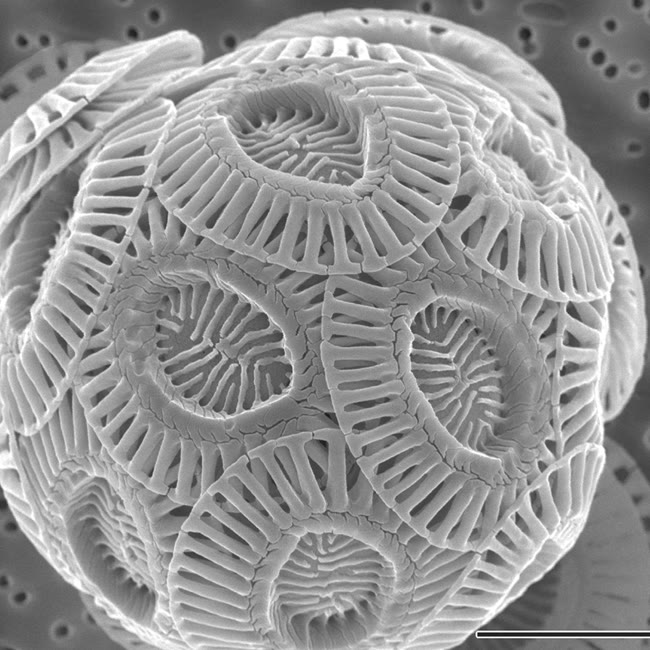
\includegraphics[height=4.3cm]{images/book3/b1-coccolithophore.jpg}};
\node[inner sep=0, anchor=west] (b) at ([xshift=0.25cm]a.east) {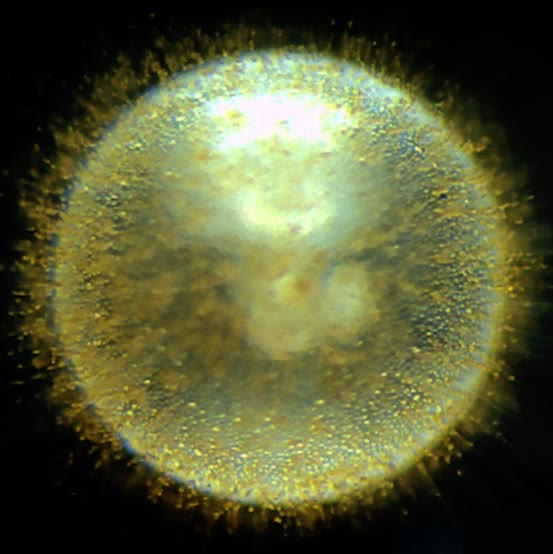
\includegraphics[height=4.3cm]{images/book3/b1-orbulina.jpg}};
\node[inner sep=0, anchor=west] (c) at ([xshift=0.25cm]b.east) {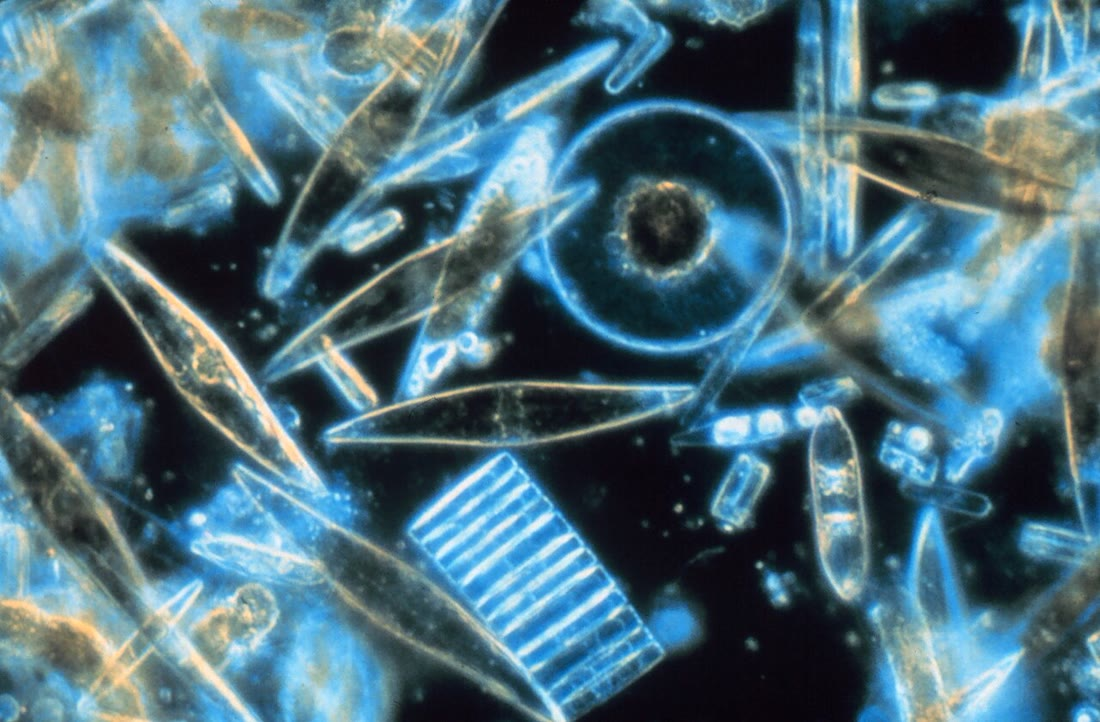
\includegraphics[height=4.3cm]{images/book3/b1-diatoms.jpg}};
\node[font=\footnotesize, anchor=north] at (a.south) {(a) un coccolithophoridé};
\node[font=\footnotesize, anchor=north] at (b.south) {(b) un foraminifère};
\node[font=\footnotesize, anchor=north] at (c.south) {(c) des diatomées};
\end{tikzpicture}

{\small Les fabricants de vases. (a)~Une cellule unique d'\emph{Emiliania huxleyi}
cuirassée de coccolithes, ses plaques de calcite (microscope électronique à balayage~;
Alison R.~Taylor, université de Caroline du Nord à Wilmington, CC~BY~2.5, via
Wikimedia Commons). (b)~Un foraminifère planctonique vivant, \emph{Orbulina
universa}, sa coquille de calcite entourée d'épines (microscope optique~; H.~Takagi
et coauteurs, 2019, CC~BY~4.0, via Wikimedia Commons). (c)~Des diatomées vivantes
de la glace de mer du détroit de McMurdo, en Antarctique, chacune dans son frustule d'opale
(microscope optique~; Gordon T.~Taylor, université Stony Brook, NOAA, domaine
public, via Wikimedia Commons).}
\label{fig:b1:chemical-biogenic-sediments:plankton}
\end{omfigure}
% ledger: commons:ehux, commons:orbulina, commons:diatoms-noaa

\begin{definition}[Lysocline, profondeur de compensation des carbonates]\label{def:b1:chemical-biogenic-sediments:ccd}
La \emph{lysocline}\index{lysocline} est la profondeur de l'océan sous laquelle la
dissolution de la calcite sur le fond marin devient d'abord visible dans le sédiment
et sa vitesse augmente brusquement. La \emph{profondeur de compensation des
carbonates}\index{profondeur de compensation des carbonates} (PCC) est la profondeur à laquelle la vitesse
de dissolution de la calcite égale la vitesse à laquelle la calcite pleut sur le fond
de la mer~; en dessous d'elle aucun carbonate de calcium ne s'accumule. En pratique on la place là où
la teneur en carbonate de calcium du sédiment de surface tombe sous \qty{10}{\%}
en masse.
\end{definition}
% ledger: slotnick:ccd-definitions

La PCC se trouve en général des centaines de mètres sous la \omterm{def:b1:chemical-biogenic-sediments:ccd}{lysocline}. Ce n'est pas un niveau
fixe~: elle est fixée par un équilibre entre apport et dissolution, si bien qu'elle est
plus profonde là où le plancton produit plus de carbonate et là où l'eau profonde est
moins corrosive. Dans l'Atlantique elle se trouve environ \qty{500}{m} plus profond que dans le
Pacifique, résultat à la fois d'un apport de carbonate plus élevé et d'une dissolution plus lente~; dans
le seul Pacifique occidental, elle se trouve à environ \qty{4000}{m} au nord-ouest et
à environ \qty{5100}{m} dans le Pacifique central. L'aragonite, plus soluble que la
calcite, se dissout à des profondeurs plus faibles encore. Au cours des temps géologiques, des variations de
l'apport, de la productivité et de la dissolution ont déplacé la PCC de plus de
\qty{2000}{m}.
% ledger: slotnick:ccd-definitions, britannica:ccd, zhang:ccd-west-pacific

\begin{method}[Localiser la lysocline et la PCC]\label{met:b1:chemical-biogenic-sediments:ccd}
\begin{enumerate}
  \item Prélever les quelques centimètres supérieurs de sédiment en des sites de profondeurs différentes
        dans une même région, assez loin de la terre et des remontées d'eau profonde pour que la dilution par
        l'argile ou par l'opale soit faible.
  \item Mesurer la teneur pondérale en \ce{CaCO3} de chaque échantillon et la porter
        en fonction de la profondeur d'eau.
  \item La \omterm{def:b1:chemical-biogenic-sediments:ccd}{lysocline} est la profondeur où la teneur commence à chuter brutalement,
        et où les coquilles montrent les premiers signes de dissolution (foraminifères
        brisés, corrodés).
  \item La PCC est la profondeur où la teneur tombe à \qty{10}{\%}~: on la lit
        par interpolation linéaire entre les deux échantillons de part et d'autre.
\end{enumerate}
\end{method}

Sur le flanc d'une dorsale médio-océanique, le fond marin est jeune et peu profond près de
l'axe et s'enfonce en vieillissant et en s'éloignant. Un morceau de fond né au-dessus de la PCC
reçoit de la \omterm{def:b1:chemical-biogenic-sediments:ooze}{vase calcaire} jusqu'à ce qu'il passe sous la PCC~; dès lors il ne reçoit
que ce qui ne se dissout pas~: la poussière qui se dépose depuis l'air au-dessus, des oxydes de fer et de
manganèse, des dents de poissons. Ce dépôt brun et lent est l'argile rouge
des bassins profonds.

\begin{proposition}[Franchir la PCC]\label{prop:b1:chemical-biogenic-sediments:flank}
Soit un fond marin d'âge $t$ à la profondeur $d(t) = d_r + C\sqrt t$
(\cref{thm:b1:rifts-ridges-margins:depth-age}), dont l'axe de dorsale à la profondeur $d_r$
est moins profond qu'une \omterm{def:b1:chemical-biogenic-sediments:ccd}{profondeur de compensation des carbonates} $z_c$ qui reste constante. Alors
le fond passe sous la PCC à l'âge
\[
t_c = \left(\frac{z_c - d_r}{C}\right)^2 ,
\]
et un site d'âge $t > t_c$ porte, de bas en haut, la \omterm{def:b1:layered-earth:layers}{croûte} volcanique,
la \omterm{def:b1:chemical-biogenic-sediments:ooze}{vase calcaire} déposée pendant le temps $t_c$, et l'argile rouge déposée pendant
le temps $t - t_c$.
\end{proposition}

\begin{proof}
La profondeur $d(t)$ croît avec $t$, et $d(t_c) = z_c$ donne $C\sqrt{t_c} =
z_c - d_r$, d'où $t_c$. Avant $t_c$ le fond se trouve au-dessus de la PCC, où
la calcite pleut plus vite qu'elle ne se dissout et où la vase s'accumule~; après $t_c$ il
se trouve en dessous, où aucun carbonate ne s'accumule et où seule s'ajoute l'argile
insoluble. La vase, une fois enterrée sous l'argile, est protégée de l'eau corrosive
au-dessus, si bien que l'ordre des couches est celui des temps.
\end{proof}

Avec $d = 2500 + 350\sqrt t$ (mètres, $t$ en millions d'années), une PCC à
\qty{4500}{m} est franchie à l'âge $(2000/350)^2 = \qty{32.7}{\Ma}$~; pour une
\omterm{def:b1:plate-kinematics:spreading-rate}{demi-vitesse d'expansion} de \qty{25}{mm} par an, cela fait \qty{816}{km} de l'axe
(figure ci-dessous). Les forages dans le vieux fond océanique
retrouvent cet ordre sans cesse~: basalte, puis \omterm{def:b1:chemical-biogenic-sediments:ooze}{vase calcaire} ou craie,
puis argile rouge, trace du voyage du fond le long du flanc. Là où la plaque
est passée depuis sous une ceinture de forte productivité, près de l'équateur, l'argile
peut être coiffée d'une nouvelle couche de vase, ce qui fait que les carottes enregistrent le mouvement des
plaques aussi bien que la profondeur de la PCC.
% ledger: parsons:plate-model

\begin{omfigure}
\begin{tikzpicture}[font=\footnotesize]
\begin{axis}[width=11cm, height=5.6cm, xmin=0, xmax=1750, ymin=2000, ymax=6200, y dir=reverse,
    xlabel={distance à l'axe de la dorsale (km), demi-vitesse d'expansion \qty{25}{mm.an^{-1}}},
    ylabel={profondeur (m)}, ytick={2000,3000,...,6000},
    axis on top, clip=false]
  % sea water above the floor
  \addplot[fill=omSea, draw=none] table[x=x_km, y=depth] {figdata/out/bachelor-1-ccd_flank-profile.dat} -- (axis cs:1750,2000) -- (axis cs:0,2000) -- cycle;
  % floor: ooze-covered above the CCD, red clay below
  \addplot[very thick, draw=omLithLime!70!black, restrict x to domain=0:816.3] table[x=x_km, y=depth] {figdata/out/bachelor-1-ccd_flank-profile.dat};
  \addplot[very thick, draw=brown!70!black, restrict x to domain=816.3:1750] table[x=x_km, y=depth] {figdata/out/bachelor-1-ccd_flank-profile.dat};
  \draw[thick, omThm, densely dashed] (axis cs:0,4500) -- (axis cs:1750,4500) node[pos=0.99, anchor=north east, inner sep=1.5pt] {PCC, \qty{4500}{m}};
  \draw[black!60, dotted, thick] (axis cs:0,4050) -- (axis cs:1750,4050) node[pos=0.99, anchor=south east, inner sep=1.5pt] {lysocline (schématique)};
  \fill[omThm] (axis cs:816.3,4500) circle[radius=2pt];
  \node[anchor=north east, align=right] at (axis cs:790,4620) {le fond franchit la PCC\\ à \qty{32.7}{\Ma}, \qty{816}{km}};
  \node[anchor=north, align=center, omLithLime!40!black] at (axis cs:520,2750) {la vase calcaire\\ s'accumule};
  \node[anchor=north west, align=left, brown!60!black] at (axis cs:1000,5180) {argile rouge sur\\ vase enterrée};
\end{axis}
% sediment column at the site 1500 km from the axis (60 Myr), schematic
\begin{scope}[xshift=10.6cm, yshift=0.4cm]
  \draw[lith basalt] (0,0) rectangle (0.9,1.0);
  \draw[lith limestone] (0,1.0) rectangle (0.9,2.6);
  \fill[brown!45, draw=black!60] (0,2.6) rectangle (0.9,3.2);
  \node[anchor=west, align=left, font=\scriptsize] at (1.0,0.5) {croûte basaltique};
  \node[anchor=west, align=left, font=\scriptsize] at (1.0,1.8) {vase calcaire\\ (0 à \qty{32.7}{\Ma})};
  \node[anchor=west, align=left, font=\scriptsize] at (1.0,2.9) {argile rouge};
  \node[anchor=south, font=\scriptsize, align=center] at (0.9,3.3) {colonne à \qty{1500}{km}\\ (schématique)};
\end{scope}
\end{tikzpicture}

{\small Les sédiments pélagiques sur un flanc de dorsale. Le fond s'approfondit avec l'âge selon la
\omterm{thm:b1:rifts-ridges-margins:depth-age}{loi profondeur--âge} $d = 2500 + 350\sqrt t$ et s'éloigne de l'axe à
\qty{25}{mm} par an~; au-dessus de la \omterm{def:b1:chemical-biogenic-sediments:ccd}{profondeur de compensation des carbonates}, prise ici à
\qty{4500}{m}, il reçoit de la \omterm{def:b1:chemical-biogenic-sediments:ooze}{vase calcaire}, en dessous seulement de l'argile rouge. Un site éloigné
de l'axe porte du basalte, de la vase et de l'argile rouge, de bas en haut (colonne à
droite, épaisseurs schématiques). La \omterm{def:b1:chemical-biogenic-sediments:ccd}{lysocline}, dessinée quelques centaines de mètres
au-dessus de la PCC, marque l'endroit où la dissolution commence à se voir.}
\label{fig:b1:chemical-biogenic-sediments:flank}
\end{omfigure}
% computed in figdata/bachelor-1/ccd_flank.py; ledger: parsons:plate-model, britannica:ccd, slotnick:ccd-definitions

\section{Les vases siliceuses et les cherts}\label{sec:b1:chemical-biogenic-sediments:silica}

Les diatomées, algues unicellulaires du plancton, et les radiolaires, membres unicellulaires
du zooplancton, bâtissent leurs squelettes d'opale, qu'ils prélèvent dans
l'acide silicique dissous dans l'eau de mer. À la différence de la calcite de l'océan de surface,
l'opale n'est pas protégée par la sursaturation~: l'eau de mer en est sous-saturée
à toutes les profondeurs, et la plus grande part de l'opale se dissout dès la mort de l'organisme,
d'abord dans l'eau pendant qu'elle coule puis sur le fond marin. Sur les 255~téramoles
de silicium incorporées chaque année à l'opale par le plancton de l'océan mondial, seules
9.2 environ sont enfouies pour de bon dans le sédiment~: une préservation de
\qty{3.6}{\%}. Un atome de silicium apporté à la mer par un fleuve est capté puis
relâché par le plancton quelque seize fois avant d'être enfoui, et il
reste environ \num{8000} ans dans l'océan.
% ledger: treguer:silica

Les \omterm{def:b1:chemical-biogenic-sediments:ooze}{vases siliceuses} se forment donc là où la production d'opale est si forte que même
\qty{3.6}{\%} d'elle finissent par compter, et où peu d'autre chose la dilue~: autour de
l'océan Austral, dans le Pacifique Nord, le long de l'équateur dans le Pacifique et sur les
marges continentales, aux endroits où l'eau profonde riche en nutriments remonte à
la surface (\cref{ch:b1:ocean-circulation}). Elles dominent aussi sous la PCC
sous des eaux productives, là où la calcite qui est tombée avec elles s'est dissoute.
% ledger: treguer:silica, og:carbonates

\begin{definition}[Chert]\label{def:b1:chemical-biogenic-sediments:chert}
Un \emph{chert}\index{chert} est une roche sédimentaire dure et dense de
quartz microcristallin, formée dans la plupart des cas à partir d'opale biogénique dissoute
puis recristallisée après enfouissement~; il se présente en bancs, souvent issus de \omterm{def:b1:chemical-biogenic-sediments:ooze}{vases siliceuses},
ou en nodules, dont le silex, dans la craie, est le plus connu.
\end{definition}
% ledger: og:carbonates

Une vase à diatomées qui n'a pas recristallisé devient une diatomite, roche légère,
blanche, poreuse, presque de l'opale pure. Avec l'enfouissement et le temps l'opale se transforme en
d'autres formes de silice et enfin en quartz, et la silice migre~: elle
quitte la craie, par exemple, et se rassemble en nodules de silex le long de certains
bancs. Comment cela se produit relève de la diagenèse (\cref{ch:b1:diagenesis-basins}).

\section{Les évaporites}\label{sec:b1:chemical-biogenic-sediments:evaporites}

Là où une masse d'eau de mer perd plus d'eau par évaporation qu'elle n'en reçoit, ses
sels se concentrent jusqu'à précipiter l'un après l'autre. La composition de
l'eau de mer est la même, pour ses ions majeurs, dans tous les océans
(\cref{tab:b1:chemical-biogenic-sediments:seawater}).

\begin{table}[htbp]
\centering\small
\begin{tabular}{@{}lrrr@{}}
\hline
ion & fraction massique du sel marin & \si{g} par \si{kg} d'eau de mer & \si{mmol} par \si{kg} \\
\hline
chlorure \ce{Cl-} & 0.5503 & 19.353 & 545.9 \\
sodium \ce{Na+} & 0.3066 & 10.781 & 469.0 \\
sulfate \ce{SO4^2-} & 0.0771 & 2.712 & 28.2 \\
magnésium \ce{Mg^2+} & 0.0365 & 1.284 & 52.8 \\
calcium \ce{Ca^2+} & 0.0117 & 0.412 & 10.3 \\
potassium \ce{K+} & 0.0113 & 0.399 & 10.2 \\
hydrogénocarbonate \ce{HCO3-} & 0.0030 & 0.105 & 1.72 \\
bromure \ce{Br-} & 0.0019 & 0.067 & 0.84 \\
\hline
tous les solutés & 1 & 35.165 & \\
\hline
\end{tabular}
\caption{Les ions majeurs de l'eau de mer de composition de référence, pour une
salinité de \qty{35.165}{g} de sel par kilogramme d'eau de mer. Le chlorure et le
sodium font \qty{86}{\%} du sel en masse~; le carbonate, le strontium, le borate et
le fluorure font l'essentiel du reste.}
\label{tab:b1:chemical-biogenic-sediments:seawater}
\end{table}
% ledger: teos10:reference-composition, teos10:reference-salinity (g and mmol computed in evaporation.py)

\begin{definition}[Évaporite, séquence d'évaporation, sabkha]\label{def:b1:chemical-biogenic-sediments:evaporite}
Une \emph{évaporite}\index{evaporite@évaporite} est un sédiment ou une roche sédimentaire de sels
précipités à partir d'une saumure naturelle concentrée par évaporation~: surtout le gypse
\ce{CaSO4.2H2O} et l'anhydrite \ce{CaSO4}, la halite \ce{NaCl}, et les sels de potassium et de
magnésium. La \emph{séquence d'évaporation}\index{sequence d'evaporation@séquence d'évaporation} est
l'ordre dans lequel les minéraux précipitent à partir de l'eau de mer qui s'évapore, le moins
soluble d'abord~: le carbonate de calcium, puis le gypse, puis la halite, puis les sels de potassium
et de magnésium. Une \emph{sabkha}\index{sabkha} est une plaine salée côtière, au niveau ou
juste au-dessus des plus hautes marées, où le gypse, l'anhydrite et la halite
croissent dans le sédiment à partir de la saumure qui s'évapore et l'imbibe.
\end{definition}
% ledger: og:carbonates, warren:brine-stages

La séquence fut observée dès 1849 par Usiglio, qui fit évaporer jusqu'à siccité un récipient
d'eau de mer~; les mesures les plus précises viennent des
salines de Great Inagua, aux Bahamas, où l'eau de mer est conduite à travers une série de
bassins de concentration croissante. Le carbonate de calcium commence à précipiter quand
la saumure est 1.8~fois plus concentrée que l'eau de mer, le gypse à 3.8~fois, la halite
à 10.6~fois~; au laboratoire le sulfate de magnésium suit vers 70~fois
et les sels de potassium au-delà de 90~fois. Les sels précipités auparavant étant une part
négligeable de la masse, un facteur de concentration de 10.6 signifie qu'il reste
$1/10.6$ de l'eau, environ \qty{9}{\%}~: la halite n'arrive que quand neuf dixièmes
de l'eau sont partis (figure ci-dessous, partie~a).
La saumure devient plus dense en se concentrant, de \qty{1.03}{g.cm^{-3}} pour
l'eau de mer à environ \num{1.13} quand le gypse se forme, \num{1.22} avec la halite et plus
de \num{1.30} avec les sels d'amertume, derniers sels de tous.
% ledger: warren:brine-stages, mccaffrey:thresholds

La quantité de chaque sel qu'un kilogramme d'eau de mer peut donner se déduit du
\cref{tab:b1:chemical-biogenic-sediments:seawater} en comptant l'ion qui s'épuise
le premier. Le carbonate de calcium est limité par le carbonate et l'hydrogénocarbonate,
\qty{1.10}{mmol}, environ \qty{0.11}{g}. Le gypse prend le calcium restant,
\qty{9.18}{mmol}, \qty{1.58}{g}, le sulfate étant en excès. La halite prend tout le
sodium, \qty{469}{mmol}, \qty{27.4}{g}, le chlorure étant en excès. Ce qui reste,
environ \qty{6.3}{g} de magnésium, de potassium, de sulfate, de chlorure et de bromure, fait
les sels d'amertume. La halite fait \qty{78}{\%} du total~: un bassin évaporitique
asséché est avant tout une masse de sel gemme.
% computed in figdata/bachelor-1/evaporation.py; ledger: teos10:reference-composition, mccaffrey:thresholds

\begin{omfigure}
\begin{tikzpicture}[font=\footnotesize]
\begin{axis}[name=a, width=7.6cm, height=5.6cm, xmode=log, xmin=1, xmax=100, ymin=0, ymax=1.05,
    xlabel={facteur de concentration de la saumure}, ylabel={fraction de l'eau restante},
    title={\footnotesize (a) seuils de la séquence d'évaporation}, grid=major, grid style={black!10},
    log ticks with fixed point]
  \addplot[omDef, thick] table[x=CF, y=f_left] {figdata/out/bachelor-1-evaporation-curve.dat};
  \addplot[omThm, only marks, mark=*, mark size=1.8pt] table[x=CF, y=f_left] {figdata/out/bachelor-1-evaporation-steps.dat};
  \node[anchor=south west, font=\scriptsize] at (axis cs:1.8,0.556) {\ce{CaCO3} (1.8)};
  \node[anchor=south west, font=\scriptsize] at (axis cs:3.8,0.263) {gypse (3.8)};
  \node[anchor=south west, font=\scriptsize] at (axis cs:10.6,0.094) {halite (10.6)};
  \node[anchor=south, font=\scriptsize, align=center] at (axis cs:60,0.16) {sels de Mg, K\\ (70, 90)};
\end{axis}
\begin{axis}[at={(a.east)}, anchor=west, xshift=1.7cm, width=7.0cm, height=5.6cm,
    ybar, bar width=14pt, ymin=0, ymax=32, xmin=0.4, xmax=4.6,
    xtick={1,2,3,4}, xticklabels={\ce{CaCO3}, gypse, halite, amertume},
    ylabel={grammes par kg d'eau de mer}, title={\footnotesize (b) masses déposées},
    nodes near coords, nodes near coords style={font=\scriptsize, /pgf/number format/precision=2},
    every node near coord/.append style={/pgf/number format/fixed}]
  \addplot[fill=omDef!40, draw=omDef] table[x=idx, y=g_per_kg] {figdata/out/bachelor-1-evaporation-masses.dat};
\end{axis}
\end{tikzpicture}

{\small L'évaporation de l'eau de mer. (a)~La fraction de l'eau restante quand la
saumure est concentrée d'un facteur donné, avec le seuil de chaque \omterm{def:b1:rock-forming-minerals:mineral}{minéral}
mesuré aux salines de Great Inagua et au laboratoire (McCaffrey,
Lazar et Holland, 1987). (b)~Les masses déposées par kilogramme d'eau de mer
évaporée jusqu'à siccité, chaque \omterm{def:b1:rock-forming-minerals:mineral}{minéral} prenant tout l'ion qui le limite
(le gypse compté avec son eau~; les sels d'amertume comptés sans la leur),
calculées à partir de la composition de référence de l'eau de mer.}
\label{fig:b1:chemical-biogenic-sediments:evaporation}
\end{omfigure}
% computed in figdata/bachelor-1/evaporation.py; ledger: mccaffrey:thresholds, teos10:reference-composition

De ces masses, l'épaisseur de sel qu'une masse d'eau donnée peut laisser
se déduit aussitôt.

\begin{proposition}[Le sel d'une colonne d'eau de mer]\label{prop:b1:chemical-biogenic-sediments:column}
Une colonne d'eau de mer de hauteur $H$ et de masse volumique $\rho_{sw}$, évaporée jusqu'à
siccité, dépose une couche d'un \omterm{def:b1:rock-forming-minerals:mineral}{minéral} de masse volumique $\rho_x$ dont l'épaisseur est
\[
h_x = \frac{\rho_{sw}\,H\,m_x}{\rho_x},
\]
où $m_x$ est la masse de ce \omterm{def:b1:rock-forming-minerals:mineral}{minéral} déposée par unité de masse d'eau de mer.
\end{proposition}

\begin{proof}
Une unité d'aire de la colonne contient la masse $\rho_{sw}H$ d'eau de mer, qui dépose
la masse $\rho_{sw}Hm_x$ du \omterm{def:b1:rock-forming-minerals:mineral}{minéral}. Étalée sur la même unité d'aire en
couche de masse volumique $\rho_x$, elle a l'épaisseur $\rho_{sw}Hm_x/\rho_x$.
\end{proof}

Avec $\rho_{sw} = \qty{1030}{kg.m^{-3}}$, $m = \qty{27.4}{g.kg^{-1}}$ et la
masse volumique de la halite, \qty{2170}{kg.m^{-3}}, une colonne d'eau de mer haute de \qty{1000}{m}
laisse \qty{13.0}{m} de halite~; avec le gypse, de masse volumique \qty{2300}{kg.m^{-3}}, elle
laisse \qty{0.71}{m} de gypse. C'est le problème d'épaisseur des \omterm{def:b1:chemical-biogenic-sediments:evaporite}{évaporites}~:
des bancs de sel épais de centaines de mètres ou de kilomètres ne peuvent être le résidu d'un
seul remplissage d'aucun bassin, si profond soit-il.
% computed in figdata/bachelor-1/evaporation.py; ledger: warren:brine-stages, webmineral:evaporites

La réponse est un bassin qui continue de recevoir de l'eau de mer. Un bassin séparé de
l'océan par un seuil, un détroit peu profond ou une barrière, sous un climat sec, perd de l'eau par
évaporation sur toute sa surface~; l'eau de mer afflue par-dessus le seuil pour la remplacer,
apportant du sel neuf, et la saumure plus dense peut ressortir en profondeur par-dessus le seuil
(figure ci-dessous). La concentration de la saumure
est fixée par l'équilibre de ces flux.

\begin{proposition}[Le bassin barré]\label{prop:b1:chemical-biogenic-sediments:barred}
Soit un bassin bien mélangé d'aire $A$ qui perd le volume $EA$ d'eau par unité de temps
par évaporation nette, reçoit de l'eau de mer au débit volumique $Q_{\mathrm{in}}$ et
rend de la saumure à l'océan au débit volumique $Q_{\mathrm{out}}$, en régime
permanent. Pour un ion qui ne précipite pas, la saumure est concentrée du
facteur
\[
k = \frac{Q_{\mathrm{in}}}{Q_{\mathrm{out}}} = \frac{Q_{\mathrm{in}}}{Q_{\mathrm{in}} - EA}
\]
par rapport à l'eau de mer (les volumes comptés comme s'ils étaient de même masse volumique).
\end{proposition}

\begin{proof}
En régime permanent le volume du bassin ne change pas, donc l'apport
équilibre la sortie et l'évaporation~: $Q_{\mathrm{in}} = Q_{\mathrm{out}} +
EA$. L'ion entre à la concentration $c_0$ de l'eau de mer et ne sort qu'avec
la saumure, à sa concentration $c$~; comme il ne précipite pas, sa masse dans
le bassin est constante quand $Q_{\mathrm{in}}c_0 = Q_{\mathrm{out}}c$. D'où $c/c_0 =
Q_{\mathrm{in}}/Q_{\mathrm{out}}$, et la substitution de $Q_{\mathrm{out}}$ donne la
seconde forme.
\end{proof}

La sortie commande ce que le bassin dépose. Si plus d'un dixième de
l'apport retourne à l'océan sous forme de saumure, $k$ reste sous 10.6 et le bassin dépose
du carbonate et du gypse mais jamais de halite~; si la sortie est plus faible, la
saumure atteint la saturation en halite et le bassin se remplit de sel~; si le détroit est
fermé tout à fait, le bassin s'assèche et son niveau baisse à la vitesse $E$.

\begin{omfigure}
\begin{tikzpicture}[font=\footnotesize, >={Stealth[length=4pt]}]
% barred evaporite basin (schematic)
\fill[omSea] (0,1.0) rectangle (3.2,3.0);
\fill[omSea!70!yellow!40] (3.6,0.6) rectangle (11.2,3.0);
\fill[omSea] (3.0,2.45) rectangle (3.8,3.0);
\draw[lith shale] (0,0) -- (0,1.0) -- (2.6,1.0) -- (3.2,2.4) -- (3.6,2.45) -- (4.4,0.6) -- (10.2,0.6) -- (11.2,2.2) -- (11.2,0) -- cycle;
\draw[lith evaporite] (4.25,0.95) -- (4.4,0.6) -- (10.2,0.6) -- (10.41,0.95) -- cycle;
\fill[omLithGranite!50, draw=black!50] (5.6,0.95) rectangle (9.0,1.35);
\draw[omSea!60!black] (0,3.0) -- (11.2,3.0);
\draw[->, thick, omDef] (1.6,2.75) -- (4.6,2.75) node[right] {apport d'eau de mer};
\draw[->, thick, omThm, densely dashed] (4.6,1.5) .. controls (4.1,2.35) and (3.8,2.57) .. (3.1,2.57) .. controls (2.6,2.57) and (2.3,2.2) .. (2.1,1.7) node[anchor=north east, inner sep=1pt] {sortie de saumure};
\foreach \x in {6.0,7.4,8.8,10.2} {\draw[->, black!60] (\x,3.1) -- (\x,3.7);}
\node[anchor=south] at (8.1,3.7) {évaporation sur le bassin};
\node at (0.8,2.15) {océan};
\node[anchor=south] at (3.4,3.0) {seuil};
\node[anchor=north, fill=white, inner sep=1pt] at (7.3,0.55) {gypse et anhydrite};
\node at (7.3,1.15) {halite};
\node at (7.3,2.2) {saumure dense};
\end{tikzpicture}

{\small Un bassin évaporitique barré (schématique)~: l'eau de mer afflue par-dessus un seuil pour
remplacer l'eau évaporée du bassin~; la saumure dense coule et une partie
retourne à l'océan en profondeur. Plus la sortie est faible, plus la
saumure est concentrée~; ici elle a dépassé la saturation en halite et la halite repose
sur le gypse antérieur.}
\label{fig:b1:chemical-biogenic-sediments:barred}
\end{omfigure}

La plus grande \omterm{def:b1:chemical-biogenic-sediments:evaporite}{évaporite} jeune du monde se trouve sous le fond de la
Méditerranée. Entre 5.97 et 5.33~millions d'années, à l'âge messinien, les
échanges d'eau entre la Méditerranée et l'Atlantique furent restreints,
et des \omterm{def:b1:chemical-biogenic-sediments:evaporite}{évaporites} épaisses jusqu'à \qty{2}{km} se déposèrent dans les bassins profonds, leur
halite surtout en un court intervalle entre 5.60 et 5.55~millions d'années. Comment
cela s'est produit est encore débattu. Dans un modèle la mer fut largement coupée et son
niveau baissa d'environ \qty{1500}{m}, les bassins profonds devenant des lacs salés et les
fleuves creusant de profonds canyons dans les marges asséchées~; dans d'autres le bassin resta
relié et plein, un bassin barré à très grande échelle. Les deux doivent expliquer
des kilomètres de sel, qu'un seul remplissage de la mer ne pourrait jamais donner.
% ledger: vasiliev:msc

\section{Exercices}

\begin{exercise}[$\star$]\label{exo:b1:chemical-biogenic-sediments:1}
L'eau de mer de composition de référence contient \qty{35.165}{g} de sel par
kilogramme, dont les fractions massiques de chlorure, de sodium, de sulfate et de magnésium
sont 0.5503, 0.3066, 0.0771 et 0.0365. Calculer la masse de chaque ion dans un kilogramme
d'eau de mer, et la fraction du sel faite de sodium et de chlorure ensemble.
% ledger: teos10:reference-composition, teos10:reference-salinity
\end{exercise}

\begin{exercise}[$\star$]\label{exo:b1:chemical-biogenic-sediments:2}
Le carbonate de calcium, le gypse, la halite et le sulfate de magnésium commencent à précipiter
à partir d'une eau de mer concentrée 1.8, 3.8, 10.6 et 70 fois. Pour chacun, calculer la
fraction de l'eau d'origine restante et la fraction déjà évaporée.
% ledger: mccaffrey:thresholds
\end{exercise}

\begin{exercise}[$\star$]\label{exo:b1:chemical-biogenic-sediments:3}
Sur les \omterm{def:b1:chemical-biogenic-sediments:reef}{récifs} que dominent les \emph{Acropora}, le bilan de carbonate est de \qty{8.4}{kg} de
\ce{CaCO3} par mètre carré et par an et le \omterm{def:b1:chemical-biogenic-sediments:reef}{récif} croît de \qty{4.2}{mm} par
an. (a)~Avec la \cref{prop:b1:chemical-biogenic-sediments:accretion}, calculer la
masse volumique sèche apparente du \omterm{def:b1:chemical-biogenic-sediments:reef}{récif}. (b)~Quelle est sa porosité si ses grains sont
d'aragonite, de masse volumique \qty{2.93}{g.cm^{-3}}~? de calcite, de masse volumique
\qty{2.71}{g.cm^{-3}}~? (c)~À même masse volumique apparente, à quelle vitesse croîtrait un \omterm{def:b1:chemical-biogenic-sediments:reef}{récif} de
bilan moyen \qty{3.7}{kg.m^{-2}.an^{-1}}~?
% ledger: perry:chagos, webmineral:polymorphs, hom:calcite
\end{exercise}

\begin{exercise}[$\star$]\label{exo:b1:chemical-biogenic-sediments:4}
Des sédiments de surface d'une région du fond océanique contiennent les
pourcentages pondéraux suivants de \ce{CaCO3}~: 88 à \qty{3000}{m}, 85 à \qty{3500}{m}, 80 à
\qty{4000}{m}, 62 à \qty{4300}{m}, 35 à \qty{4500}{m}, 12 à \qty{4700}{m}, 6
à \qty{4800}{m} et 2 à \qty{5000}{m}. Avec la
\cref{met:b1:chemical-biogenic-sediments:ccd}, situer la \omterm{def:b1:chemical-biogenic-sediments:ccd}{lysocline} et la PCC.
\end{exercise}

\begin{exercise}[$\star\star$]\label{exo:b1:chemical-biogenic-sediments:5}
(a)~Écrire l'équation équilibrée de la précipitation du carbonate de calcium à partir des
ions calcium et hydrogénocarbonate, et calculer la masse de dioxyde de carbone
libérée par kilogramme de \ce{CaCO3} déposé (masses molaires \qty{100.09}{g.mol^{-1}}
et \qty{44.01}{g.mol^{-1}}). (b)~Combien libérerait, d'après cette
équation, un \omterm{def:b1:chemical-biogenic-sediments:reef}{récif} de bilan \qty{3.7}{kg.m^{-2}.an^{-1}} par mètre carré et par an~?
(c)~Pourquoi un \omterm{def:b1:chemical-biogenic-sediments:reef}{récif}, qui transforme du carbone dissous en roche, libère-t-il du
dioxyde de carbone~?
% ledger: perry:chagos
\end{exercise}

\begin{exercise}[$\star\star$]\label{exo:b1:chemical-biogenic-sediments:6}
Prendre le fond marin à la profondeur $d = 2500 + 350\sqrt t$ (mètres, $t$ en
millions d'années), s'éloignant de sa dorsale à la demi-vitesse de \qty{25}{mm} par
an. (a)~À quel âge et à quelle distance de l'axe franchit-il une PCC à
\qty{4500}{m}~? (b)~Même question pour une PCC à \qty{5100}{m}, comme dans le Pacifique
central. (c)~Pendant combien de temps un fond de \qty{60}{\Ma} aurait-il reçu de l'argile rouge dans
chaque cas~?
% ledger: parsons:plate-model, zhang:ccd-west-pacific
\end{exercise}

\begin{exercise}[$\star\star$]\label{exo:b1:chemical-biogenic-sediments:7}
Un \omterm{def:b1:chemical-biogenic-sediments:reef}{récif} croît de \qty{4.2}{mm} par an. (a)~Peut-il suivre une
montée relative du niveau de la mer de \qty{3}{mm} par an~? (b)~Son sommet se trouve à \qty{2}{m} sous
la mer quand la montée relative devient \qty{10}{mm} par an. Si ses bâtisseurs ne peuvent
vivre plus profond que \qty{50}{m}, au bout de combien de temps se noie-t-il~?
(c)~Pourquoi peut-il en fait se noyer plus tôt~?
% ledger: perry:chagos
\end{exercise}

\begin{exercise}[$\star\star$]\label{exo:b1:chemical-biogenic-sediments:8}
Enfoui sous quelques centaines de mètres de sédiments, le gypse \ce{CaSO4.2H2O}
(\qty{172.17}{g.mol^{-1}}, masse volumique \qty{2.30}{g.cm^{-3}}) perd son eau et
devient de l'anhydrite \ce{CaSO4} (\qty{136.14}{g.mol^{-1}}, masse volumique
\qty{2.97}{g.cm^{-3}}). (a)~Écrire la réaction. (b)~Calculer les volumes molaires des
deux minéraux et la variation de volume du solide. (c)~Quelle fraction de
la masse du gypse part sous forme d'eau~? Que peut faire cette eau dans les roches
environnantes~?
% ledger: webmineral:evaporites
\end{exercise}

\begin{exercise}[$\star\star$]\label{exo:b1:chemical-biogenic-sediments:9}
Le plancton de l'océan mondial incorpore 255~téramoles de silicium à l'opale par
an, et 9.2 sont enfouies. (a)~Calculer la fraction préservée et la fraction
dissoute. (b)~Pourquoi une \omterm{def:b1:chemical-biogenic-sediments:ooze}{vase siliceuse} peut-elle néanmoins se former, et où~? (c)~Pourquoi
l'enregistrement des diatomées dans le sédiment donne-t-il une image biaisée des diatomées qui
ont vécu dans l'eau~?
% ledger: treguer:silica
\end{exercise}

\begin{exercise}[$\star\star\star$]\label{exo:b1:chemical-biogenic-sediments:10}
Un bassin barré d'aire \qty{10000}{km^2} perd par évaporation nette \qty{1.5}{m}
d'eau par an. (a)~Calculer le volume évaporé chaque année. (b)~Avec la
\cref{prop:b1:chemical-biogenic-sediments:barred}, calculer le facteur de concentration
de la saumure quand l'apport par-dessus le seuil est de \qty{1.8e10}{m^3} par an,
et quand il est de \qty{1.575e10}{m^3} par an. Quels minéraux peuvent précipiter dans
chaque cas~? (c)~Jusqu'à quel apport le bassin dépose-t-il de la halite~?
% ledger: mccaffrey:thresholds
\end{exercise}

\begin{exercise}[$\star\star\star$]\label{exo:b1:chemical-biogenic-sediments:11}
L'eau de mer contient \qty{0.0673}{g} de bromure par kilogramme. Quand la halite
précipite, elle capte du bromure en proportion de sa concentration dans la
saumure~: la teneur en bromure de la halite vaut $D = 0.032$ fois celle de la
saumure. (a)~Calculer la teneur en bromure de la saumure, en milligrammes par
kilogramme, et de la première halite, quand la saumure est 10.6~fois plus concentrée que
l'eau de mer. (b)~Même question quand la saumure a atteint 30~fois. (c)~Le bromure est
à peine retiré de la saumure par la halite~: pourquoi~? (d)~Dans un banc épais de halite,
la teneur en bromure croît vers le haut, puis retombe brusquement. Que s'est-il passé dans
le bassin~?
% ledger: teos10:reference-composition, mccaffrey:dbr, mccaffrey:thresholds
\end{exercise}

\begin{exercise}[$\star\star\star$]\label{exo:b1:chemical-biogenic-sediments:12}
Un site sur le flanc d'une dorsale est à la profondeur $d = 2500 + 350\sqrt t$ et a maintenant
\qty{70}{\Ma}. Supposer que la \omterm{def:b1:chemical-biogenic-sediments:ooze}{vase calcaire} s'accumule à \qty{2}{cm} par
millier d'années au-dessus de la PCC et l'argile rouge à \qty{1}{mm} par millier d'années
en dessous, et négliger la compaction. (a)~Calculer l'épaisseur de vase et d'argile
rouge sur le site pour une PCC à \qty{4500}{m}. (b)~Même question pour une PCC
\qty{500}{m} plus profonde, comme dans l'Atlantique. (c)~Une carotte du site montre une mince
couche de vase au sein de l'argile rouge. Donner deux explications possibles.
% ledger: parsons:plate-model, britannica:ccd
\end{exercise}

\section{Problème~: Le sel d'une mer disparue}

\begin{problem}[{Problème du week-end --- quelle quantité d'eau de mer il faut pour faire un bassin de sel,
et en combien de temps}]
\label{pb:b1:chemical-biogenic-sediments:1}
% values: calc/ch22.py; the basin, its area, inflow and evaporation are invented
Une mer intérieure d'aire $A = \qty{1.0e5}{km^2}$, profonde de \qty{1000}{m}, est reliée à
l'océan par un détroit au-dessus d'un seuil peu profond. Son fond, aujourd'hui enfoui, porte
\qty{1.5}{km} de halite. Prendre pour l'eau de mer la masse volumique \qty{1030}{kg.m^{-3}} et
les masses déposées par kilogramme calculées dans le chapitre~: \qty{0.110}{g} de
\ce{CaCO3}, \qty{1.581}{g} de gypse, \qty{27.41}{g} de halite et
\qty{6.34}{g} de sels d'amertume~; pour les minéraux les masses volumiques~: calcite
\qty{2710}{kg.m^{-3}}, gypse \qty{2300}{kg.m^{-3}}, anhydrite
\qty{2970}{kg.m^{-3}}, halite \qty{2170}{kg.m^{-3}}. Traiter la mer comme une boîte à
parois verticales.

\medskip
\noindent\textbf{Partie I --- Un remplissage.}
\begin{enumerate}
  \item Calculer la masse d'eau de mer au-dessus d'un mètre carré de fond, et
        la masse de sel qu'elle contient (\qty{35.165}{g.kg^{-1}}).
  \item Calculer la masse de gypse et de halite déposée sur un mètre carré
        quand la mer s'évapore jusqu'à siccité.
  \item Avec la \cref{prop:b1:chemical-biogenic-sediments:column}, calculer
        l'épaisseur de carbonate de calcium, de gypse et de halite.
  \item Enfoui, le gypse devient de l'anhydrite. Quelle est alors l'épaisseur de la
        couche de sulfate~?
  \item Quelle fraction du sel sec est de la halite~? Pourquoi une mer asséchée est-elle surtout
        du sel gemme~?
  \item Dans quel ordre, de bas en haut, les couches se superposent-elles~? Pourquoi~?
\end{enumerate}

\noindent\textbf{Partie II --- La saumure à mesure que la mer s'assèche.}
\begin{enumerate}[resume]
  \item À quelle profondeur de saumure, dans la boîte, le carbonate de calcium, le gypse et la
        halite commencent-ils à précipiter~?
  \item Quelle fraction de l'eau s'est évaporée quand la halite apparaît~?
  \item Sous quelle profondeur de saumure les sels de magnésium et de potassium commencent-ils~?
  \item Quelle est la masse volumique de la saumure à chaque stade~? Qu'est-ce que cela implique pour une saumure
        qui rencontre de l'eau de mer fraîche affluant~?
  \item Pourquoi le premier dépôt, le carbonate, se voit-il rarement comme une couche séparée
        dans un bassin évaporitique~?
  \item La teneur en bromure de la halite croît de la base au sommet de
        la couche de halite d'un remplissage. Pourquoi~?
\end{enumerate}

\noindent\textbf{Partie III --- Combien de remplissages~?}
\begin{enumerate}[resume]
  \item Combien de remplissages du bassin, évaporé à chaque fois jusqu'à siccité, faudrait-il
        pour déposer les \qty{1.5}{km} de halite~?
  \item Quelle quantité d'anhydrite l'accompagnerait, et comment serait-elle
        répartie dans la coupe~?
  \item Quelle serait l'épaisseur des sels d'amertume, s'ils étaient tous conservés, avec une
        masse volumique moyenne de \qty{2000}{kg.m^{-3}}~? Pourquoi manquent-ils si souvent~?
  \item Comment la teneur en bromure de la halite enregistrerait-elle chaque nouveau remplissage~?
  \item Les \omterm{def:b1:chemical-biogenic-sediments:evaporite}{évaporites} messiniennes atteignent \qty{2}{km}. Combien de remplissages d'une
        mer de \qty{1000}{m} leur halite exigerait-elle, si elles étaient entièrement de halite~?
\end{enumerate}

\noindent\textbf{Partie IV --- Apport et temps.}
\begin{enumerate}[resume]
  \item L'eau de mer afflue par-dessus le seuil à \qty{5000}{m^3.s^{-1}} et aucune saumure
        ne ressort~; le niveau reste constant. Calculer le taux d'évaporation nette
        sur la mer, en mètres par an (une année de $365.25$ jours).
  \item Calculer la masse de sel qui entre dans la mer chaque année.
  \item Si toute sa halite se dépose uniformément sur le fond, quelle épaisseur de halite
        se forme chaque année~?
  \item Combien de temps les \qty{1.5}{km} de halite mettent-ils à se former~?
  \item Le détroit se ferme. À quelle vitesse le niveau baisse-t-il, et au bout de combien de temps
        la mer est-elle asséchée, si le taux d'évaporation reste le même~?
  \item Combien de temps après la fermeture la halite commence-t-elle à précipiter~?
  \item À l'entier le plus proche, combien de remplissages du bassin son
        sel a-t-il exigé~?
\end{enumerate}
\end{problem}
